% $HeadURL$

\subsection{Glyph: \glyph{Source} and \glyph{Sink}}
\label{sec:sourceSink}

It is useful to have the ability to represent the creation of an entity or
a state from an unspecified source, that is, from something that one does
not need or wish to make precise.  For instance, in a model where the
production of a protein is represented, it may not be desirable to
represent all of the amino acids, sugars and other metabolites used, or the
energy involved in the protein's creation.  Similarly, we may not wish to
bother representing the details of the destruction or decomposition of some
biochemical species into a large number of more primitive entities,
preferring instead to simply say that the species ``disappears into a
sink''.  Yet another example is that one may need to represent an input
(respectively, output) into (resp. from) a compartment without explicitly
representing a transport process from a source (resp. to a target).

For these and other situations, SBGN defines two glyphs that use the same symbol for explicitly
representing the involvement of an unspecified source or sink.  The symbol
used in SBGN is borrowed from the mathematical symbol for ``empty set'',
but it is important to note that it does not actually represent a true
absence of everything or a physical void---it represents the absence of the
corresponding structures in the model, that is, the fact that these sources
or sinks are conceptually outside the scope of the map. The reason that we
regard the \glyph{Source} and \glyph{Sink} as different glyphs is that they have different
syntax and semantics (the former only connects to a \glyph{Consumption} arc and the latter
a \glyph{Production} arc). This is mainly an issue for software tools and those mapping to
and from SBGN from other notations of exchange formats.

A frequently asked question is, why bother having an explicit symbol at
all?  The reason is that one cannot simply use an arc that does not
terminate on a node, because the dangling end could be mistaken to be
pointing to another node in the map.  This is specially true if the
map is rescaled, causing the spacing of elements in the map to
change.  The availability and use of an explicit symbol for sources and
sinks is critical.

\begin{glyphDescription}

\glyphSboTerm SBO:0000291 ! empty set

\glyphContainer A \glyph{source} or \glyph{sink} is represented by the mathematical symbol for ``empty
set'', that is, a circle crossed by a bar linking the upper-right and
lower-left corners of an invisible square drawn around the circle ($\emptyset$).
\fig{sourceSink} illustrates this.  The symbol should be linked to one
and only one edge in a map.

\glyphLabel A \glyph{source} or \glyph{sink} does not carry any labels.

\glyphAux A \glyph{source} or \glyph{sink} does not carry any auxiliary items.  

\end{glyphDescription}

\begin{figure}[H]
  \centering
  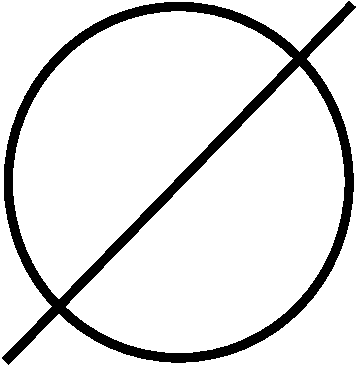
\includegraphics[scale = 0.3]{images/build/sourceSink.pdf}
  \caption{The \glyph{source} and \glyph{sink} glyphs.}
  \label{fig:sourceSink}
\end{figure}






% The following is for [X]Emacs users.    Please leave in place.
% Local Variables:
% TeX-master: "../sbgn_PD-level1"
% End:
